\chapter{Mapping}
\label{sec:mapping}

\section{Mapping files}
Mapping relates atomistic and coarse-grained representations of the system. It is organized as follows: for each molecule {\em type} a mapping file is created. When used as a command option, these files are combined in a list separated by a semicolon, e.~g. \progopt{--cg}~\texttt{"protein.xml;solvent.xml"}.

Each mapping file contains a {\em topology} of the coarse-grained molecule and a list of {\em maps}. Topology specifies coarse-grained beads and bonded interactions between them. Each coarse-grained bead has a name, type, a list of atoms which belong it, and a link to a map. A map is a \hyperref[sec:mapping_operator]{set of weights} $c_{Ii}$ for an atom $i$ belonging to the bead $I$. It is used to calculate the position of a coarse-grained bead from the positions of atoms which belong to it. Note that $c_{Ii}$ will be automatically re-normalized if their sum is not equal to 1, i.~e. in the case of a center-of-mass mapping one can simply specify atomic masses.
A complete reference for mapping file definitions can be found in sec.~\ref{sec:ref_mapping}.

As an example, we will describe here a mapping file of a united atom model of a propane molecule. In this coarse-grained model two bead types (A,B) and three beads (A1, B1, A2) are defined, as shown in fig.~\ref{fig:propane_map}. We will use centers of mass of the beads as  coarse-grained coordinates.


\begin{figure}[ht]
  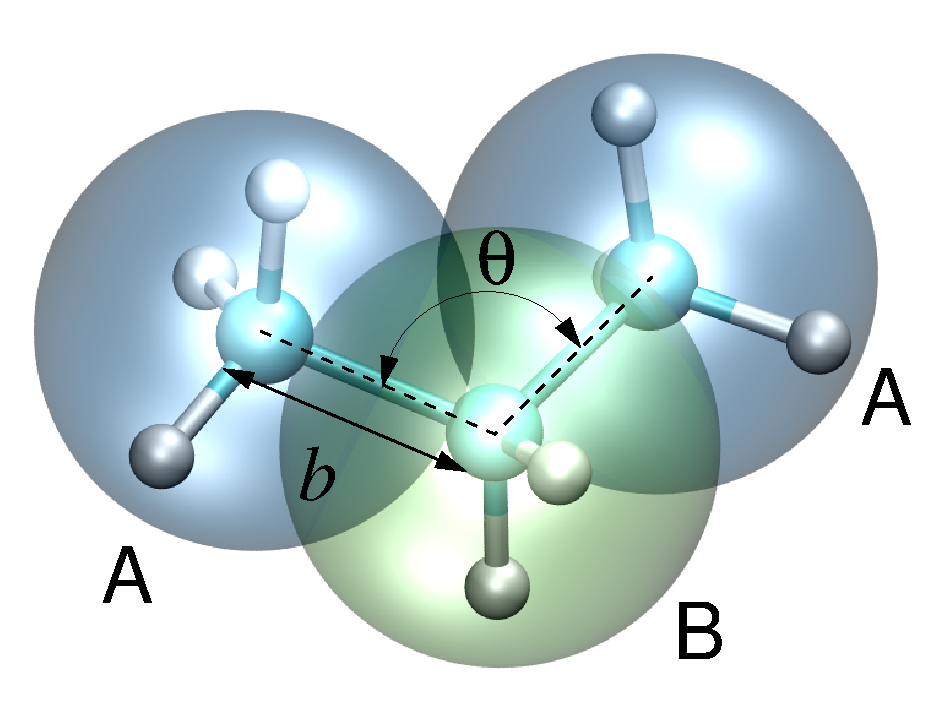
\includegraphics[width=0.4\textwidth]{functionality/fig/propane.eps}
  \caption{Mapping for propane
  \label{fig:propane_map}
}
\end{figure}

\lstinputlisting{functionality/propane.xml}

The \mapopt{ident} tag in the mapping definition must match the name of the molecule in the reference system.

The name must be unique within the mapping file. Type defines the type of the bead. The \hyperlink{\mapref{topology.cg_beads.cg_bead.mapping}}{mapping} tag defines which mapping scheme is used from the mapping section in the file.

Type and mapping can be different since the number of atoms for the same bead type may differ, e.g. at chain ends for saturating hydrogen atoms.

In the \hyperlink{\mapref{topology.cg_beads.cg_bead.mapping}}{mapping section}, the mapping operator is defined. Currently this includes only weights for a linear mapping scheme.

To map from an atomistic to a reference system, \prog{csg_map} can be used:
\begin{verbatim}
  csg_map --top topol.tpr --trj traj.trr --cg "protein.xml;solvent.xml" --out cg.gro
\end{verbatim}

To create a coarse-grained topology based on the mapping scheme, see \prog{csg_gmxtopol}.



\section{Advanced topology handling}
\label{sec:adv_topology}


A topology is defined as a set of beads with a certain bead type which are connected by bonded interactions.
\votca can read topologies in the \gromacs tpr format. However, it can also use a pdb file as topology, but, not all information are given or defined in this file format. If a pdb topology is used, it is recommended to fill in any additional molecule information using the xml advanced topology handling feature (see. \sect{sec:adv_topology})


Many file formats do not have a clear definition of molecules. This can lead to problems, especially if a simulation contains several molecules with multiple types. Since during the coarse graining, the molecule type is identified by a name tag, names must also be set properly. \votca also offers the possibility to read a topology and later on modify parts of it. Everything is based on a definition in an \xml topology file. This new \xml topology can then be used as topology in the \progopt{--tpr} option, as any other topology file.

As \gromacs did not store molecule names in previous versions, but has introduced this feature in a newer release,  a recent .tpr file which contains molecule names should always be provided. For old topologies, rerun \gromacs \progex{grompp} if possible to get a recent file.

If no molecule information is present at all, it has to be manually defined. An example for a topology file that reads in last.pdb and then creates proper molecule definitions is:
\begin{lstlisting}
<topology base="last.pdb">
  <molecules>
    <clear/>
    <define name="mCP" first="1" nbeads="52" nmols="216"/>
  </molecules>
</topology>
\end{lstlisting}
where $<$clear/$>$ clears all molecule information that were present before.

If molecule information is already present in the parent topology, but molecule do not have proper names, molecules can be renamed. A short example is
\begin{lstlisting}
 <topology base="topol.tpr">
   <molecules>
     <rename name="PPY3" range="1:125"/>
     <rename name="Cl" range="126:250"/>
   </molecules>
 </topology>
\end{lstlisting}
Here, first the file topol.tpr is loaded, subsequently, molecules are renamed.

\section{Trajectories}
A trajectory is defined as a set of frames containing coordinates and eventually velocities and forces for the beads of a topology.
\votca currently supports trr, xtc, pdb and gro as trajectory formats.





